%  article.tex (Version 3.3, released 19 January 2008)
%  Article to demonstrate format for SPIE Proceedings
%  Special instructions are included in this file after the
%  symbol %>>>>
%  Numerous commands are commented out, but included to show how
%  to effect various options, e.g., to print page numbers, etc.
%  This LaTeX source file is composed for LaTeX2e.

%  The following commands have been added in the SPIE class
%  file (spie.cls) and will not be understood in other classes:
%  \supit{}, \authorinfo{}, \skiplinehalf, \keywords{}
%  The bibliography style file is called spiebib.bst,
%  which replaces the standard style unstr.bst.
\RequirePackage{snapshot}
\newcommand{\argmin}[1]{\underset{#1}{\operatorname{arg}\,\operatorname{min}}\;}

\documentclass[12pt]{spieman}
%%\documentclass[letter]{spie}  %>>> use for US letter paper
%%\documentclass[a4paper]{spie}  %>>> use this instead for A4 paper
%%\documentclass[nocompress]{spie}  %>>> to avoid compression of citations
%% \addtolength{\voffset}{9mm}   %>>> moves text field down
%\renewcommand{\baselinestretch}{1.65}   %>>> 1.65 for double spacing, 1.25 for 1.5 spacing


\makeatletter
\@fpsep\textheight
\makeatother


%% Latex documents that need direct input
\title{Non Destructive Testing based on a Scanning-From-Heating approach: Application to non-through defect detection and fiber orientation assessment}

\author[a]{Belkacemi M.}
\author[a]{Stolz C.}
\author[b]{Mathieu A.}
\author[a,c]{Lemaitre G.}
\author[a]{Massich J.}
\author[a]{Aubreton O.}
\affil[a]{LE2I UMR6306, CNRS, Arts et M\'etiers, Univ. Bourgogne Franche-Comt\'e, 12 rue de la Fonderie, Le Creusot, France, 71200}
\affil[b]{ICB, UMR 6303 CNRS-Universit\'e Bourgogne Franche-Comt\'e, 12 rue de la Fonderie, Le Creusot, France, 71200}
\affil[c]{ViCOROB, Universitat de Girona, Campus Montilivi, Edifici P4, Girona, Spain, 17071}




%  The following command loads a graphics package to include images
%  in the document. It may be necessary to specify a DVI driver option,
%  e.g., [dvips], but that may be inappropriate for some LaTeX
%  installations.
\usepackage{subfigure}
\usepackage[]{graphicx}

% In order to include files without having a clear page using \include*,
% the newclude package is required
\usepackage{newclude}

% Required for acronyms
% use \acresetall to reset the acroyms counter
% macros=True, allows for calling \myTriger rather than \ac{myTriger}
\usepackage[single=true, macros=true, xspace=true]{acro}

% In SPIE template, biblatex can NOT be used to manage the referencing
%
%\usepackage[style=spiebib, backend=biber]{biblatex}

% Clever cross referencing. Using cleverref, instead of writting
% figure~\ref{...} or equation~\ref{...}, only \cref{...} is required.
% The package interprates the references and introduces the figure, fig.,
% equation, eq., etc keywords. \Cref forces first letter capital.
% >> WARNING: This package needs to be loaded after hyperref, math packages,
%             etc. if used.
%             Cleveref is recomended to load late
\usepackage{hyperref}
\usepackage{cleveref}

% To create random text use lipsum
\usepackage{lipsum}

% math package
\usepackage{amsmath,amsfonts, amssymb}

% units package
\usepackage{siunitx}
%array
\usepackage{multirow}

% acronym
\usepackage{acro}

% Include the following packages to use tikz
\usepackage{tikz,xifthen}
\usepackage{tikz-qtree}
\usetikzlibrary{decorations.pathmorphing} % noisy shapes
\usetikzlibrary{fit}% fitting shapes to coordinates
\usetikzlibrary{backgrounds}% drawing the background after the foreground
\usetikzlibrary{shapes,arrows,shadows}
\usetikzlibrary{calc,decorations.pathreplacing,decorations.markings,positioning}
\usetikzlibrary{snakes,decorations.text,shapes,patterns}
\usepackage{transparent}

\usepackage[skins]{tcolorbox}        % contains the latex packages
%\input{content/frontmatter.tex}             % contains the Title and Autor info
%\input{latex/filesystem/fileSetup.tex}      % contains package and variables init.
%% Acronym definition example using glossaries package
%% \usepackage{acro} is required
%% 
%% For a powerful usage of the acro package look at http://tex.stackexchange.com/questions/135975/how-to-define-an-acronym-by-using-other-acronym-and-print-the-abbreviations-toge

\DeclareAcronym{ndt}{
  short = NDT ,
  long = Non-Destructive Testing
}

\DeclareAcronym{sfh}{
  short = SFH,
  long = Scanning-From-Heating
}

\DeclareAcronym{pt}{
  short = PT,
  long = Pulse Thermography
}

\DeclareAcronym{ppt}{
  short = PPT,
  long = Pulse Phase Thermography
}

\DeclareAcronym{lt}{
  short = LT,
  long = Lock-in Thermography
}

\DeclareAcronym{fem}{
  short = FEM,
  long = Finite Element Method
}

\DeclareAcronym{sthm}{
  short = SThM,
  long = Thermal Scanning Microscope
}

\DeclareAcronym{sem}{
  short = SEM,
  long = Scanning Electron Microscope
}

\DeclareAcronym{roi}{
  short = ROI,
  long = Region Of Interest
}      % contains the acronims

%% Select inputing only one part of the document
%\includeonly{content/intro/intro}   % the file wihtout .tex
%\includeonly{content/other/other_content}

% \addbibresource{./content/lit_review.bib}
% \addbibresource{./content/biblatex-examples.bib}

\begin{document}

\maketitle

\begin{abstract}
\acresetall  % reset the acronyms from the title (if any)
Nowadays, industries ensure the quality of their manufactured products through computer vision techniques and non-conventional imaging. 3D scanners and \ac{ndt} systems are commonly used independently for such applications. Furthermore, these approaches combined together constitute a hybrid systems providing a 3D reconstruction and \ac{ndt} analysis. These systems, however, suffer from drawback such as errors during the data fusion and higher cost for manufacturers. In an attempt to solve those problems, a single active thermography system based on \ac{sfh} is proposed in this paper. Besides 3D digitization of the object, our contributions are twofold: (i) the non-through defect detection for homogeneous metallic object and (ii) fiber orientation assessment for long fiber composite material. The experiments on steel and aluminum plates show that our method achieves to detect non-through defects. Additionally, the estimation of the fiber orientation is evaluated on carbon-fiber composite material.
\end{abstract}

\keywords{Non Destructive Testing, Active Thermography, 3D scanning, Fiber orientation, Non-through defect detection}


%>>>> Include contact information for corresponding author
{\noindent \footnotesize\textbf{*} Mohamed Belkacemi, \linkable{Mohamed.Belkacemi@u-bourgogne.fr} }

%%%%%%%%%%%%%%%%%%%%%%%%%%%%%%%%%%%%%%%%%%%%%%%%%%%%%%%%%%%%%

\begin{spacing}{2}   % use double spacing for rest of manuscript

%%%%%%%%%%%%%%%%%%%%%%%%%%%%%%%%%%%%%%%%%%%%%%%%%%%%%%%%%%%%%

%% Incldue the content without .tex extension
\acresetall  % reset the acronyms from the abstract
\include*{content/intro/intro}          % the file wihtout .tex
\include*{content/rel/rel}
\include*{content/simu/simu}
\include*{content/exp/exp}
\include*{content/conc/conc}
% \include*{content/other/other}

\acknowledgments     %>>>> equivalent to \section*{ACKNOWLEDGMENTS}

This work is supported by the Regional Council of Burgundy. We are extremely grateful to members of laboratory LE2I for day to day help and collaboration.


\newpage
\bibliography{./Bibliography}   %>>>> bibliography data in report.bib
\bibliographystyle{spiejour}   %>>>> makes bibtex use spiebib.bst


\newpage
\input{./content/biography/biography.tex} 

\newpage
\listoffigures

\newpage
\listoftables

\newpage \graphicspath{ {./Figure/Figure6/} }
\begin{figure}
  \centering
  \hspace*{\fill}
  %\subfigure[]{\label{subfig:4a}\includegraphics[width=0.3\linewidth]{fig4a.png}} \hfill
  %\subfigure[]{\label{subfig:4b}\includegraphics[width=0.3\linewidth]{fig4b.png}} 
  %\hspace*{\fill} \\ \hspace*{\fill}
  %\subfigure[]{\label{subfig:4c}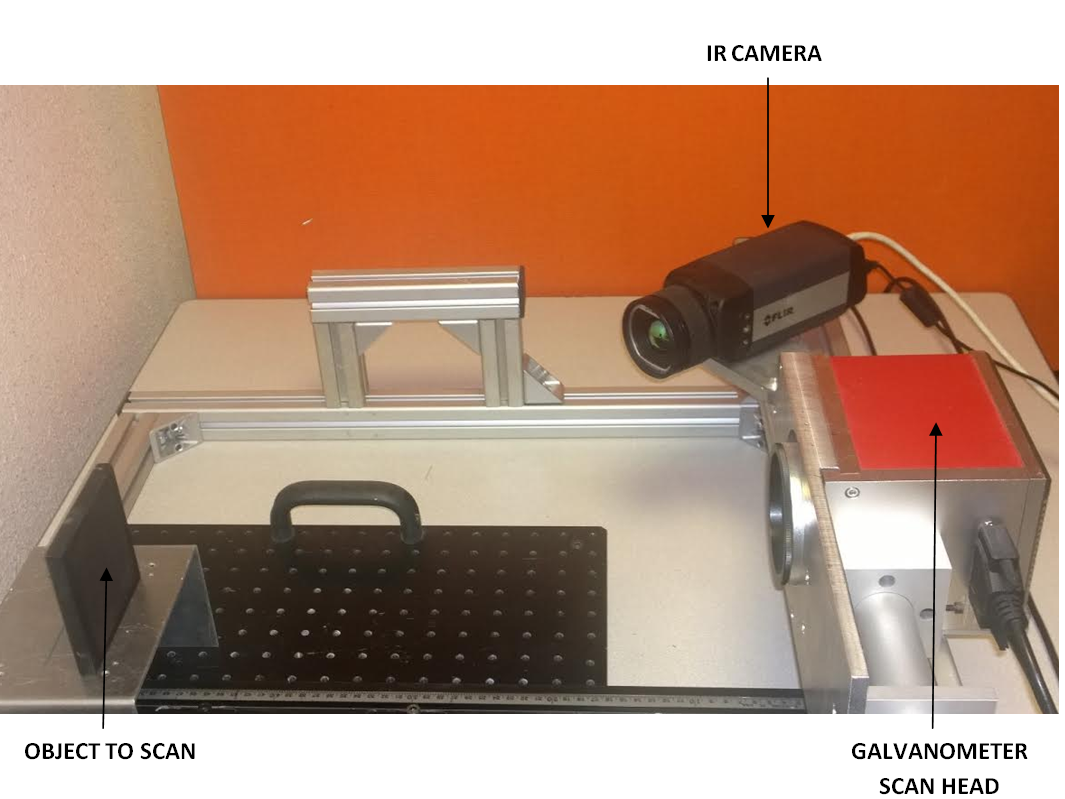
\includegraphics[width=0.3\linewidth]{fig4c.png}}
	{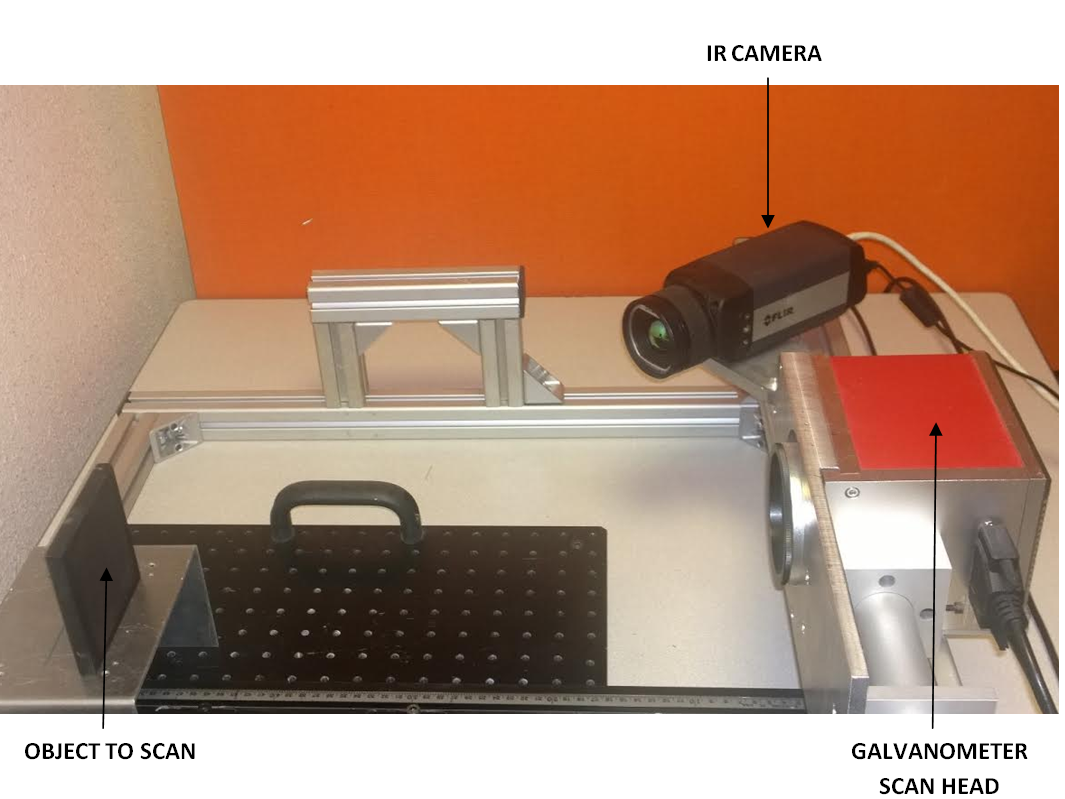
\includegraphics[width=0.7\linewidth]{fig4c.png}}
  \hspace*{\fill}
	
	\caption{Scanner prototype.}
  \label{fig:4}
\end{figure}
  

\newpage \graphicspath{ {./Figure/Figure7/} }
\begin{figure}
  \centering
	
  \hspace*{\fill}
  \subfigure[]{\label{subfig:44a}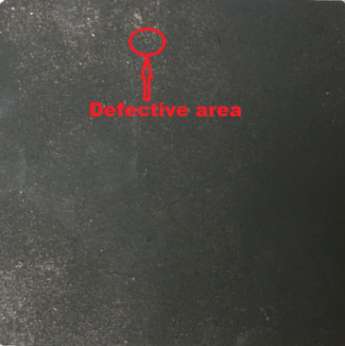
\includegraphics[width=0.3\linewidth]{fig3a.png}} \hfill
  \subfigure[]{\label{subfig:44b}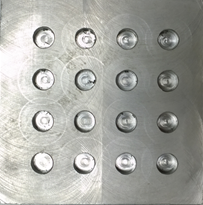
\includegraphics[width=0.3\linewidth]{fig3b.png}} 
  \hspace*{\fill} \\ \hspace*{\fill}
  \subfigure[]{\label{subfig:44c}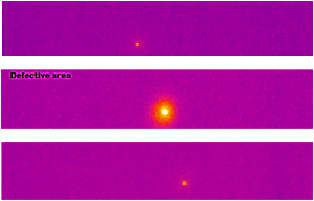
\includegraphics[width=0.3\linewidth]{fig3c.png}}
  %\subfigure[]{\label{subfig:3d}\includegraphics[width=0.3\linewidth]{fig3d.png}}
  \hspace*{\fill}
	
	  \caption{(a) Front side of the inspected material - (b) Back side of the inspected
		material - (c) Form of the thermal response of the material in the area with and without
		defect.}
		\label{fig:44}
		\end{figure}
  

\newpage \graphicspath{ {./Figure/Figure8/}}
\begin{figure}
  \centering
	

  \hspace*{\fill}
  %\subfigure[]{\label{subfig:6a}\includegraphics[width=0.3\linewidth]{fig6a.png}} \hfill
  %\subfigure[]{\label{subfig:6b}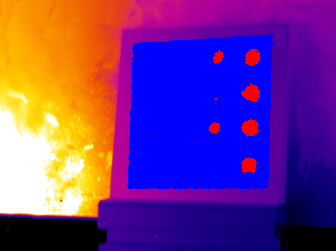
\includegraphics[width=0.3\linewidth]{fig6b.png}} 
  \subfigure[]{\label{subfig:6a}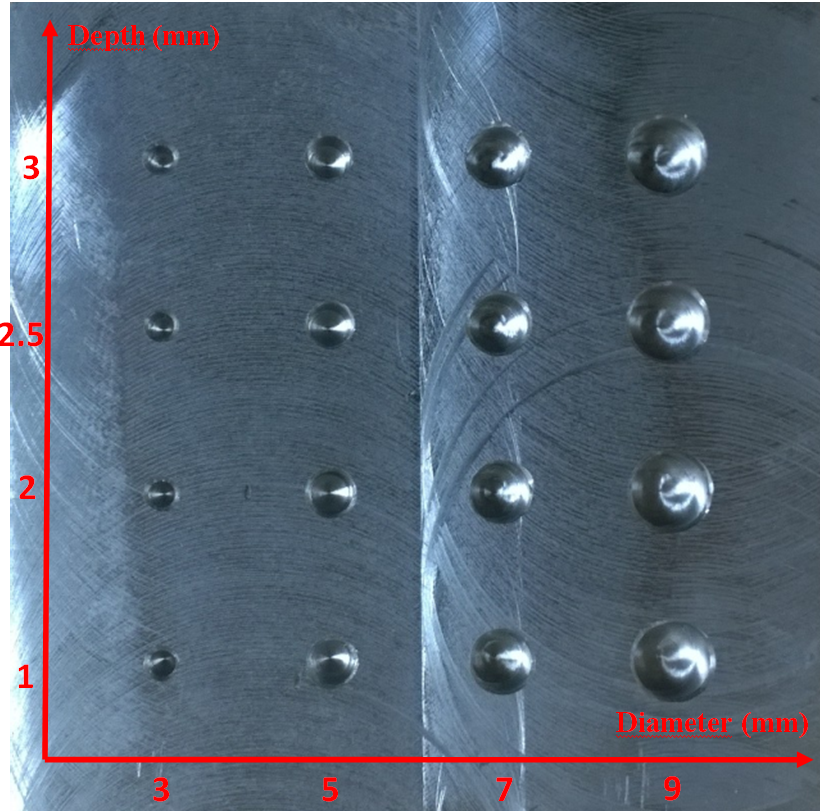
\includegraphics[width=0.3\linewidth]{fig7b.png}} \hfill
	\subfigure[]{\label{subfig:6b}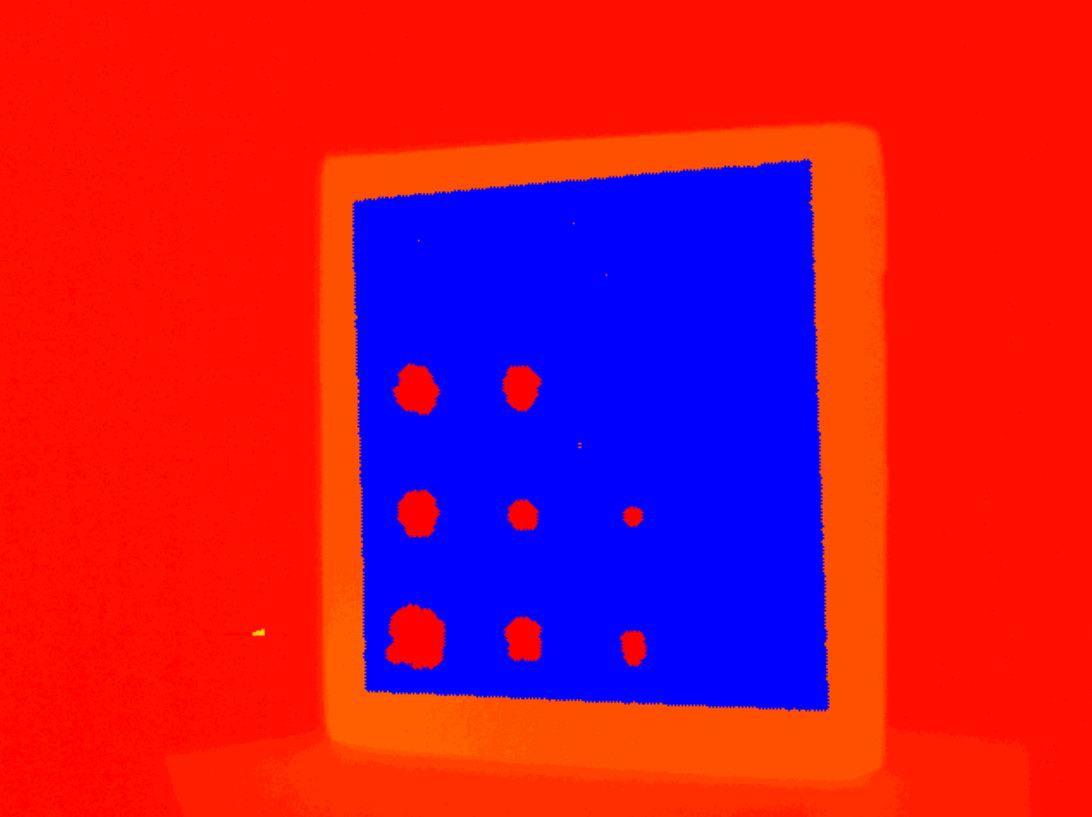
\includegraphics[width=0.3\linewidth]{fig7c.png}}
  \hspace*{\fill} \\ \hspace*{\fill}
  \subfigure[]{\label{subfig:6c}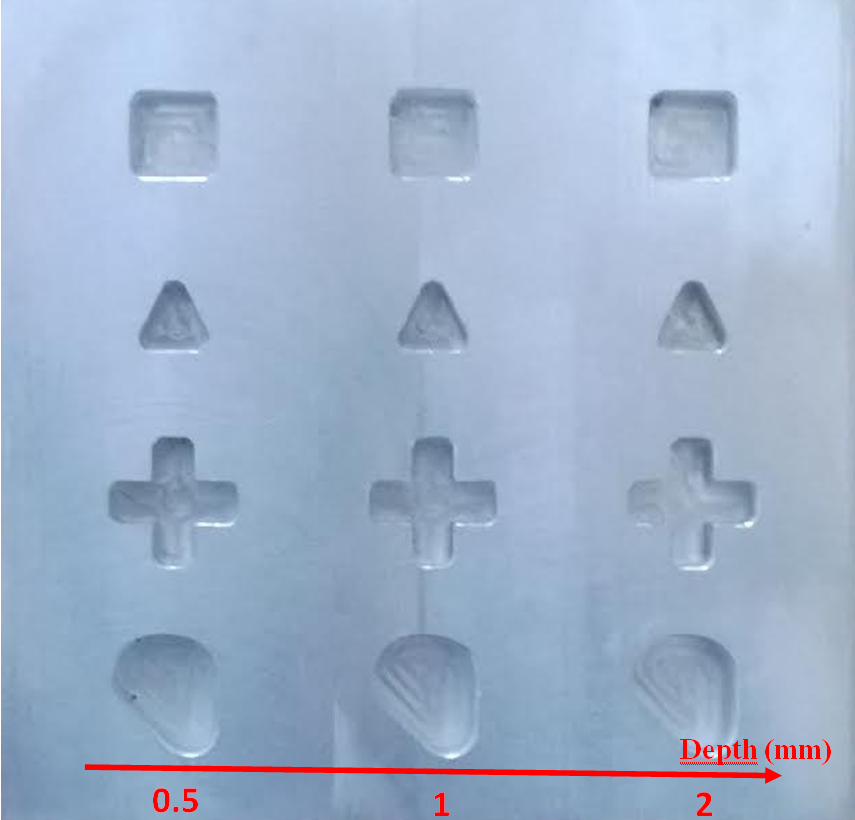
\includegraphics[width=0.3\linewidth]{fig6c.png}} \hfill
  \subfigure[]{\label{subfig:6d}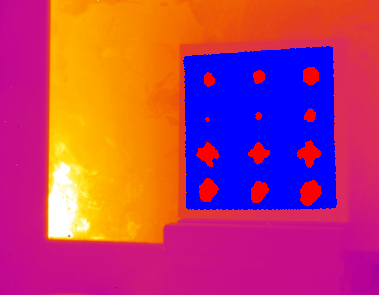
\includegraphics[width=0.3\linewidth]{fig6d.png}}
  \hspace*{\fill}
	
	  \caption{(a) and (c) Steel and aluminum objects - (b) and (d) Corresponding detection map.}
		\label{fig:6}
		\end{figure}
  

\newpage \graphicspath{ {./Figure/Figure9/}}
\begin{figure}
  \centering
	

  \hspace*{\fill}
  \subfigure[]{\label{subfig:7a}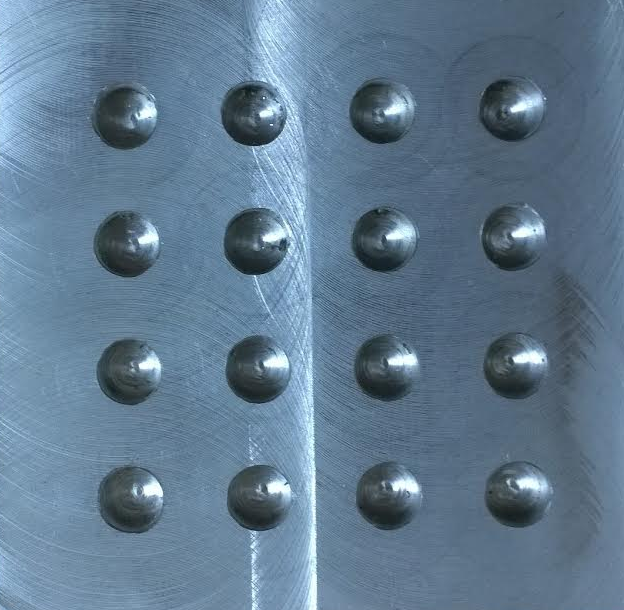
\includegraphics[width=0.3\linewidth]{fig7a.png}} \hfill
	\subfigure[]{\label{subfig:7b}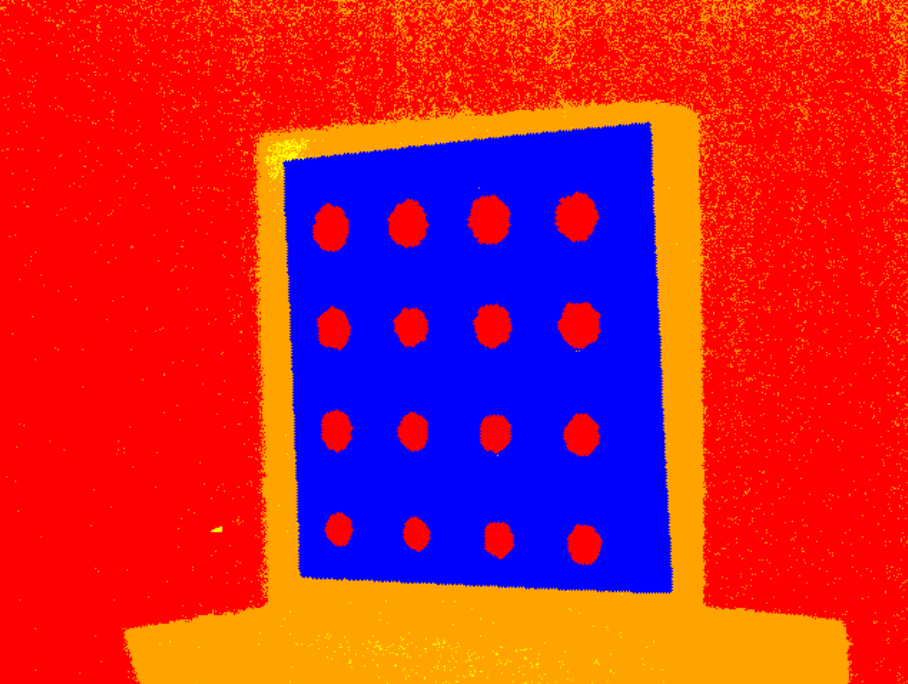
\includegraphics[width=0.3\linewidth]{fig7d.png}} 
  \hspace*{\fill}


	
		\caption{(a) Steel objects - (b) Corresponding detection map.}
  \label{fig:7}
\end{figure}
  

\newpage \graphicspath{ {./Figure/Figure10/}}
\begin{figure}
  \centering
	
  \hspace*{\fill}
  \subfigure[]{\label{subfig:8a}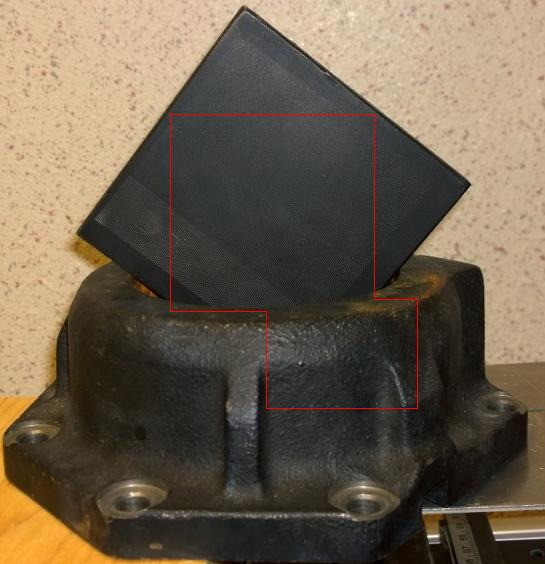
\includegraphics[width=0.3\linewidth]{fig8a.png}}\hfill
  \subfigure[]{\label{subfig:8b}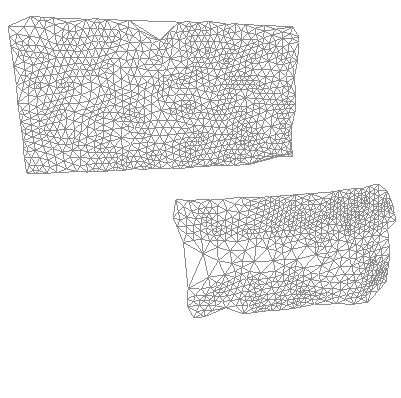
\includegraphics[width=0.3\linewidth]{fig8b.png}} 
	\hspace*{\fill} \\ \hspace*{\fill}
  \subfigure[]{\label{subfig:8c}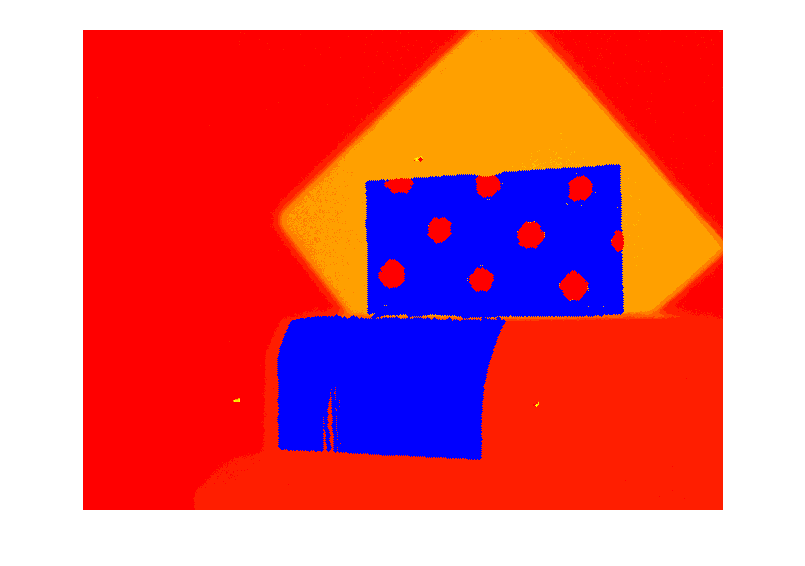
\includegraphics[width=0.3\linewidth]{fig8c.png}} \hfill
  \subfigure[]{\label{subfig:8d}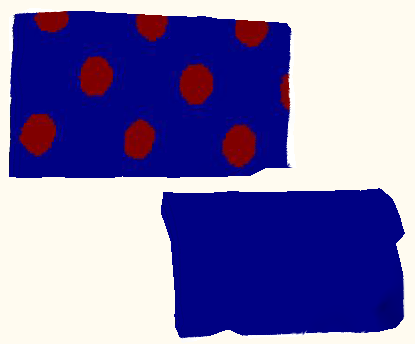
\includegraphics[width=0.3\linewidth]{fig8d.png}}
  \hspace*{\fill}
	
	\caption{(a) The specimen - (b) 3D mesh - (c) Corresponding detection map - (d) 3D mapping.}
  \label{fig:8}
\end{figure}
 

\newpage \graphicspath{ {./Figure/Figure11/}}
\begin{figure}
  \centering
	

  \hspace*{\fill}
  \subfigure[]{\label{subfig:9a}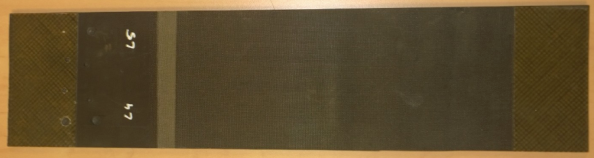
\includegraphics[width=0.3\linewidth]{fig9a.png}}
  \hspace*{\fill} \\ \hspace*{\fill}
  \subfigure[]{\label{subfig:9b}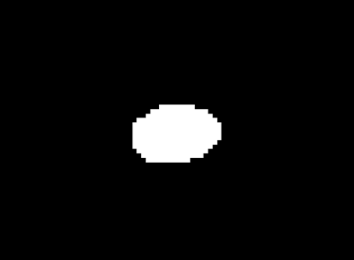
\includegraphics[width=0.3\linewidth]{fig9b.png}} \hfill
  \subfigure[]{\label{subfig:9c}
\includegraphics[width=0.3\linewidth]{fig9c.png}} \hfill
  \subfigure[]{\label{subfig:9d}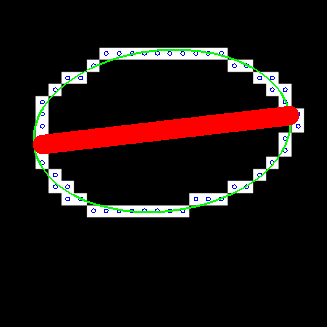
\includegraphics[width=0.3\linewidth]{fig9d.png}}
  \hspace*{\fill}
	  
		\caption{(a) The specimen - (b) Segmented thermal response - (c) Edge of the thermal
		response - (d) Ellipse fitting.}
		\label{fig:9}
		\end{figure}
  

\newpage \graphicspath{ {./Figure/Figure12/}}
\begin{figure}
  \centering

  \hspace*{\fill}
  \subfigure[]{\label{subfig:10a}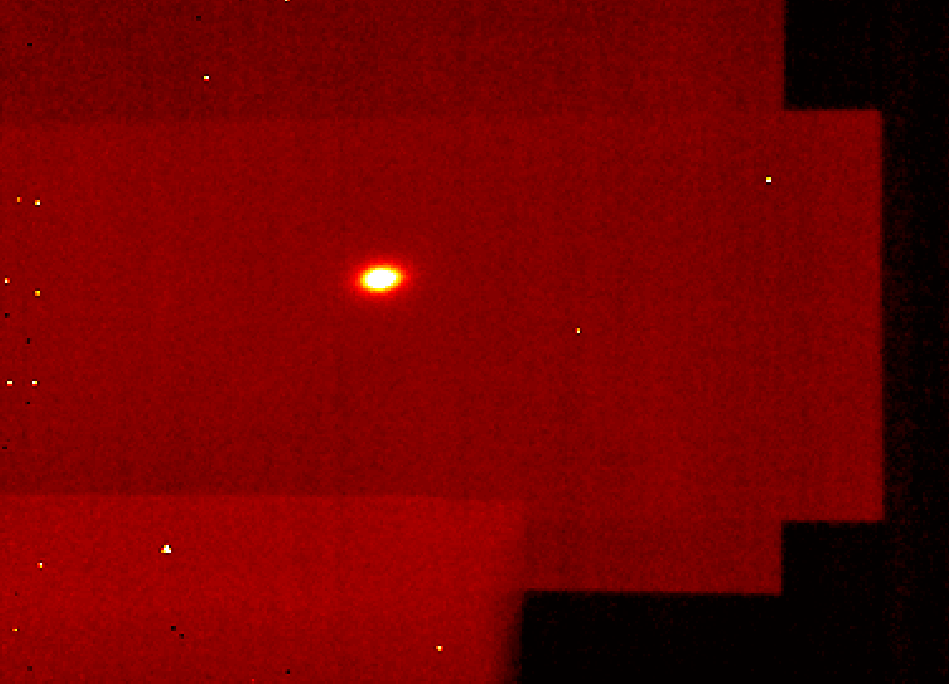
\includegraphics[width=0.3\linewidth]{fig10aa.png}} \hfill
  \subfigure[]{\label{subfig:10b}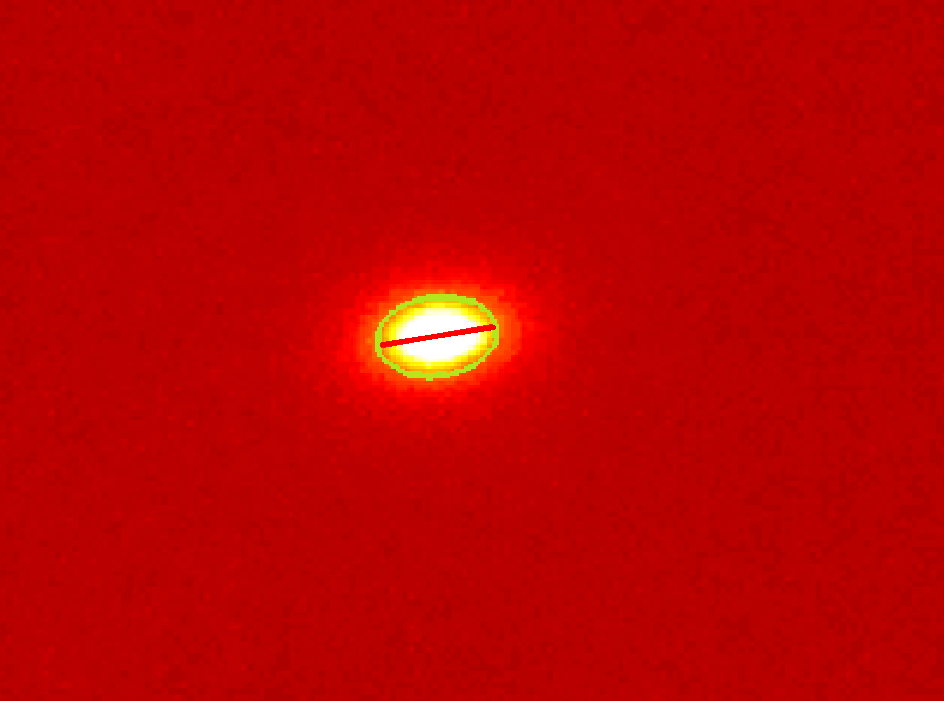
\includegraphics[width=0.3\linewidth]{fig10bb.png}} 
  \hspace*{\fill} \\ \hspace*{\fill}
  \subfigure[]{\label{subfig:10c}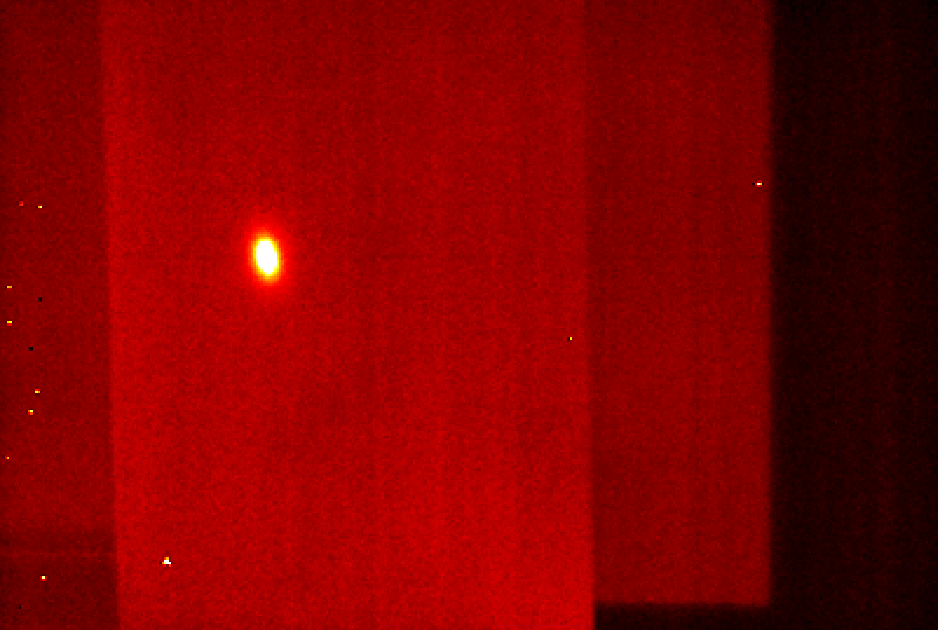
\includegraphics[width=0.3\linewidth]{fig10cc.png}} \hfill
  \subfigure[]{\label{subfig:10d}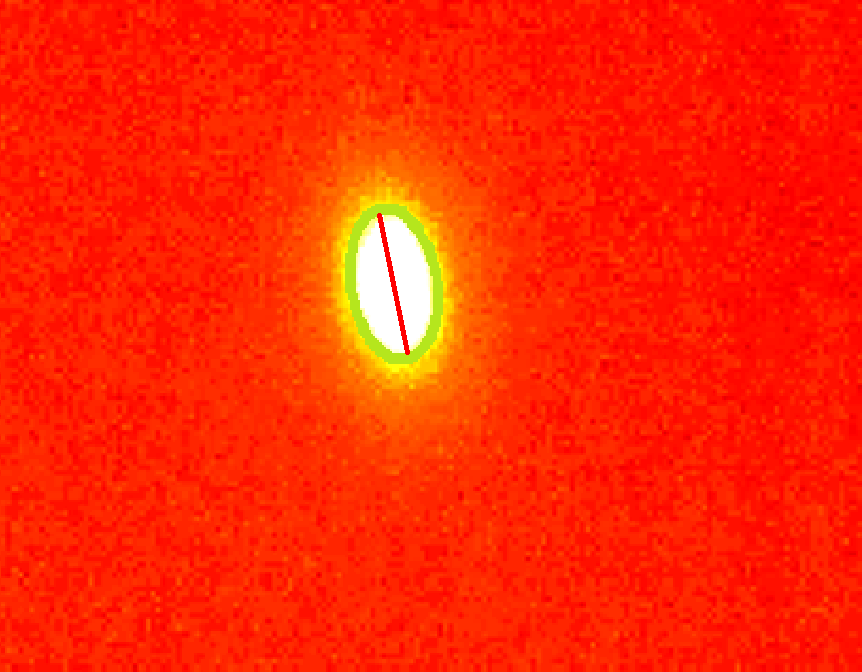
\includegraphics[width=0.3\linewidth]{fig10dd.png}}
  \hspace*{\fill}
	
	\caption{Example of fiber orientation detection: (a)-(b) horizontally oriented - (c)-(d)
		vertically oriented.}
		\label{fig:10}
		\end{figure}
  


\end{spacing}
\end{document}


%%% Local Variables:
%%% mode: latex
%%% TeX-master: t
%%% End:
